% -----------------------------------------------------------------------------
% bob: an FPGA built inside an FPGA -- project presentation (Beamer)
%
% Self-contained: every figure is TikZ, no image files. Compiles with pdfLaTeX
% (e.g. on Overleaf: New Project > Upload > this file, compiler pdfLaTeX).
% Every number comes from the project's own records: docs/project/REPORT.md,
% docs/reports/M*/ (Vivado), docs/hwtest/results.log (board runs), device.json.
% Fill in \author and \institute below.
% -----------------------------------------------------------------------------
\documentclass[aspectratio=169,11pt]{beamer}

\usepackage[T1]{fontenc}
\usepackage{lmodern}
\usepackage{booktabs}
\usepackage{tikz}
\usetikzlibrary{arrows.meta,positioning,shapes.geometric,calc,fit,backgrounds}

% --- look ------------------------------------------------------------------------
\usetheme{default}
\definecolor{bobteal}{HTML}{0C7A64}
\definecolor{bobamber}{HTML}{E38A1F}
\definecolor{bobviolet}{HTML}{6A4DB3}
\definecolor{bobink}{HTML}{16202B}
\definecolor{bobmute}{HTML}{566372}
\definecolor{bobpanel}{HTML}{F2F5F8}
\definecolor{bobclb}{HTML}{DFE7EF}
\definecolor{bobbram}{HTML}{D9ECF7}
\definecolor{bobdsp}{HTML}{F5E4D6}
\definecolor{bobio}{HTML}{E9E4F3}
\setbeamercolor{structure}{fg=bobteal}
\setbeamercolor{normal text}{fg=bobink}
\setbeamercolor{frametitle}{fg=bobink}
\setbeamercolor{alerted text}{fg=bobamber}
\setbeamerfont{frametitle}{series=\bfseries,size=\Large}
\setbeamertemplate{navigation symbols}{}
\setbeamertemplate{itemize items}[circle]
\setbeamertemplate{footline}{%
  \hfill{\scriptsize\color{bobmute}bob: an FPGA inside an FPGA\quad\insertframenumber/\inserttotalframenumber}\hspace*{1em}\vspace*{0.6em}}
\newcommand{\kpi}[2]{\begin{tabular}{@{}c@{}}{\Large\bfseries\color{bobteal}#1}\\[-2pt]{\scriptsize\color{bobmute}#2}\end{tabular}}
\newcommand{\src}[1]{{\scriptsize\color{bobmute}#1}}

\tikzset{
  blk/.style={draw=bobink!60, fill=bobpanel, rounded corners=2pt, align=center, font=\small, minimum height=8mm},
  hot/.style={draw=bobamber, fill=bobamber!15, rounded corners=2pt, align=center, font=\small, minimum height=8mm},
  acc/.style={draw=bobteal, fill=bobteal!12, rounded corners=2pt, align=center, font=\small, minimum height=8mm},
  cfg/.style={draw=bobviolet, fill=bobviolet!12, rounded corners=2pt, align=center, font=\small, minimum height=8mm},
  arr/.style={-{Stealth[length=2mm]}, thick, color=bobink!70},
}

\title{bob: an FPGA built inside an FPGA}
\subtitle{A complete, programmable FPGA with its own configuration logic and tool chain,\\running on a PYNQ-Z2 (Zynq XC7Z020)}
\author{Your Name}            % <- fill in
\institute{Your Institute}    % <- fill in
\date{September 2026}

\begin{document}

% =============================================================================
\begin{frame}[plain]
  \titlepage
\end{frame}

% =============================================================================
\begin{frame}{The idea in one picture}
  \centering
  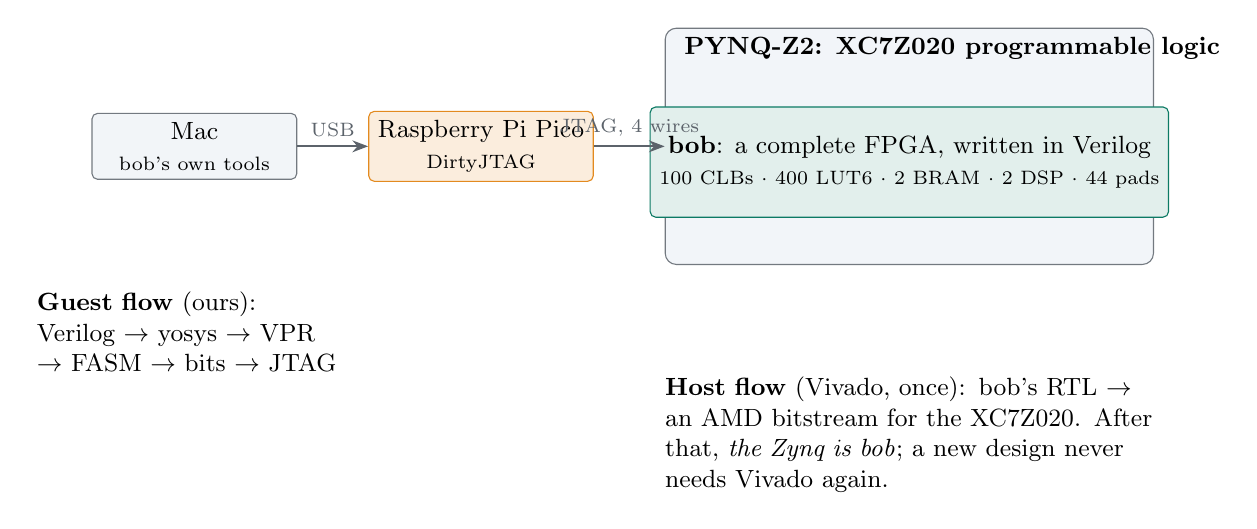
\begin{tikzpicture}[node distance=6mm and 9mm]
    \node[blk, minimum width=26mm] (mac) {Mac\\\scriptsize bob's own tools};
    \node[hot, right=of mac, minimum width=22mm] (pico) {Raspberry Pi Pico\\\scriptsize DirtyJTAG};
    \node[draw=bobink!60, rounded corners, right=of pico, minimum width=62mm, minimum height=30mm, fill=bobclb!40] (pynq) {};
    \node[anchor=north west, font=\small\bfseries] at (pynq.north west) {\ PYNQ-Z2: XC7Z020 programmable logic};
    \node[acc, minimum width=48mm, minimum height=14mm] at ($(pynq.center)+(0,-2mm)$) (bob) {\textbf{bob}: a complete FPGA, written in Verilog\\\scriptsize 100 CLBs $\cdot$ 400 LUT6 $\cdot$ 2 BRAM $\cdot$ 2 DSP $\cdot$ 44 pads};
    \draw[arr] (mac) -- node[above,font=\scriptsize]{USB} (pico);
    \draw[arr] (pico) -- node[above,font=\scriptsize]{JTAG, 4 wires} (pynq);
    \node[below=13mm of mac, text width=40mm, font=\small, align=left] (g) {\textbf{Guest flow} (ours):\\ Verilog $\rightarrow$ yosys $\rightarrow$ VPR\\ $\rightarrow$ FASM $\rightarrow$ bits $\rightarrow$ JTAG};
    \node[below=13mm of pynq, text width=62mm, font=\small, align=left] (h) {\textbf{Host flow} (Vivado, once): bob's RTL $\rightarrow$ an AMD bitstream for the XC7Z020. After that, \emph{the Zynq is bob}; a new design never needs Vivado again.};
  \end{tikzpicture}
  \vspace{2mm}

  \small Every layer an FPGA vendor hides (the fabric, the configuration memory, the configuration controller, the bitstream format and the tools) is built here, open, and checked.
\end{frame}

% =============================================================================
\begin{frame}{Outline}
  \begin{columns}[T]
    \column{0.48\textwidth}
    \begin{enumerate}
      \item Goals and the rules of the work
      \item The device: CLB, routing, BRAM, DSP, pads
      \item Configuration: JTAG, packets, frames, the ``brain''
      \item The tool chain: Verilog to a running design
      \item Timing without a timing model
    \end{enumerate}
    \column{0.48\textwidth}
    \begin{enumerate}\setcounter{enumi}{5}
      \item Software: the CLI and bob studio
      \item Verification, from unit benches to the board
      \item Growing the grid: 16 to 400 LUTs
      \item Results, problems and lessons
      \item Limits and future work
    \end{enumerate}
  \end{columns}
\end{frame}

% =============================================================================
\section{Goals}
\begin{frame}{Goals and the rules of the work}
  \begin{columns}[T]
    \column{0.5\textwidth}
    \textbf{Goals}
    \begin{itemize}
      \item A \alert{real} FPGA: logic, memory, DSP, routing, I/O
      \item Configured like a real one: AMD UG470-style frames and packets over JTAG
      \item Its own tools: synthesis, place and route, bitstream, timing
      \item Everything proven: on the board, not only in simulation
    \end{itemize}
    \column{0.5\textwidth}
    \textbf{Rules}
    \begin{itemize}
      \item Follow the references (AMD UG470/473/474/479, OpenFPGA, VPR) and say where bob diverges
      \item One milestone at a time; each ends with a \alert{hardware test} on the PYNQ-Z2
      \item Every hardware check first gets a passing \emph{and} a failing case against a software stand-in board
      \item Architecture numbers live in one file (\texttt{device.py}); everything else is generated
    \end{itemize}
  \end{columns}
  \vspace{3mm}
  \centering
  \kpi{26}{milestones, M0--M25}\qquad
  \kpi{71/71}{board checks at M25}\qquad
  \kpi{$\approx$40k}{lines of code}\qquad
  \kpi{12 days}{Sep 14--26, 2026}
\end{frame}

% =============================================================================
\section{The device}
\begin{frame}{The device at a glance (M25, on the board)}
  \begin{columns}[c]
    \column{0.52\textwidth}
    \centering
    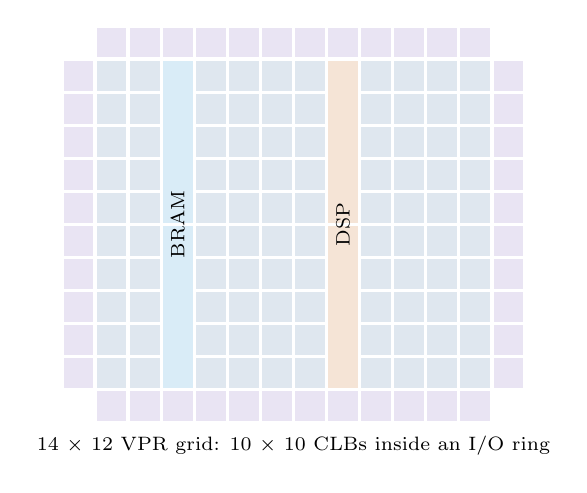
\begin{tikzpicture}[x=4.2mm,y=4.2mm]
      % 14 x 12 grid: io ring, CLB core, BRAM column x=3, DSP column x=8
      \foreach \x in {1,...,12} { \fill[bobio] (\x+0.05,0.05) rectangle (\x+0.95,0.95); \fill[bobio] (\x+0.05,11.05) rectangle (\x+0.95,11.95); }
      \foreach \y in {1,...,10} { \fill[bobio] (0.05,\y+0.05) rectangle (0.95,\y+0.95); \fill[bobio] (13.05,\y+0.05) rectangle (13.95,\y+0.95); }
      \foreach \x in {1,2,4,5,6,7,9,10,11,12} \foreach \y in {1,...,10}
        { \fill[bobclb] (\x+0.05,\y+0.05) rectangle (\x+0.95,\y+0.95); }
      \fill[bobbram] (3.05,1.05) rectangle (3.95,5.95); \fill[bobbram] (3.05,6.05) rectangle (3.95,10.95);
      \fill[bobdsp] (8.05,1.05) rectangle (8.95,5.95); \fill[bobdsp] (8.05,6.05) rectangle (8.95,10.95);
      \node[font=\scriptsize, rotate=90] at (3.5,6) {BRAM};
      \node[font=\scriptsize, rotate=90] at (8.5,6) {DSP};
      \node[font=\scriptsize] at (7,-0.7) {14 $\times$ 12 VPR grid: 10 $\times$ 10 CLBs inside an I/O ring};
    \end{tikzpicture}
    \column{0.46\textwidth}
    \small
    \begin{tabular}{@{}ll@{}}
      \toprule
      CLBs & 100 $\times$ 4 elements = \textbf{400 LUT6} \\
      Element & fracturable LUT6, carry, 2 FFs, Double Duty \\
      CLB & N = 4, I = 16, full crossbar \\
      BRAM & 2 $\times$ 1024 $\times$ 18, true dual port (UG473) \\
      DSP & 2 slices, 25 $\times$ 18 MAC, P48 (UG479) \\
      Routing & L4, W = 36, Wilton, 5\,695 muxes \\
      Pads & 44, boundary scan \\
      Config & \textbf{532 frames = 68\,096 bits} \\
      IDCODE & \texttt{0x0B025093} \\
      \bottomrule
    \end{tabular}
    \vspace{2mm}

    \src{Host cost: 38\,198 LUTs (71.8\%) and 86.8\% of the XC7Z020's slices.}
  \end{columns}
\end{frame}

% =============================================================================
\begin{frame}{The logic element and the CLB}
  \begin{columns}[c]
    \column{0.55\textwidth}
    \centering
    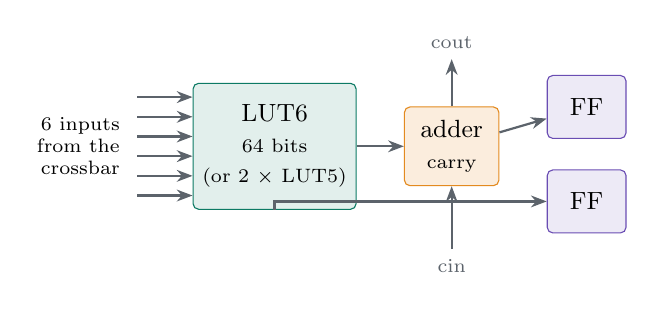
\begin{tikzpicture}[font=\small]
      \node[acc, minimum width=18mm, minimum height=16mm] (lut) {LUT6\\\scriptsize 64 bits\\\scriptsize (or 2 $\times$ LUT5)};
      \node[hot, right=6mm of lut, minimum width=12mm, minimum height=10mm] (add) {adder\\\scriptsize carry};
      \node[cfg, right=6mm of add, minimum width=10mm, yshift=5mm] (ff1) {FF};
      \node[cfg, right=6mm of add, minimum width=10mm, yshift=-7mm] (ff2) {FF};
      \draw[arr] (lut) -- (add); \draw[arr] (add) -- (ff1); \draw[arr] (lut.south) |- (ff2);
      \draw[arr] ($(add.south)+(0,-8mm)$) node[below,font=\scriptsize]{cin} -- (add.south);
      \draw[arr] (add.north) -- ++(0,6mm) node[above,font=\scriptsize]{cout};
      \foreach \i in {0,...,5} \draw[arr] ($(lut.west)+(-7mm,{0.25*(\i-2.5)})$) -- ($(lut.west)+(0,{0.25*(\i-2.5)})$);
      \node[left=8mm of lut, font=\scriptsize, align=right] {6 inputs\\from the\\crossbar};
    \end{tikzpicture}
    \column{0.43\textwidth}
    \small
    \begin{itemize}
      \item Element after UG474 / OpenFPGA \texttt{k6\_frac\_N10}: LUT6 or two LUT5s, a carry bit, flip-flops with enable and sync reset/set
      \item \alert{Double Duty} (Pun et al., FPL 2025, M24): the adder takes two inputs directly, so the LUT stays free: 4.7\% fewer elements (VPR), 13.2\% (bob's packer)
      \item CLB: 4 elements behind a \textbf{full crossbar}; N and crossbar population chosen by a measured sweep (M21)
    \end{itemize}
  \end{columns}
\end{frame}

% =============================================================================
\begin{frame}{Routing generated from VPR's own graph}
  \begin{columns}[c]
    \column{0.5\textwidth}
    \small
    \begin{itemize}
      \item VPR describes the architecture as a \textbf{routing-resource graph} (rr graph): every wire and pin a node, every switch an edge
      \item \texttt{fabric\_gen.py} (the OpenFPGA method) turns \alert{every node with fan-in into a multiplexer} in the RTL
      \item So VPR routes on \emph{exactly} the hardware that exists; there is nothing to keep in sync
      \item Routing muxes are built from host LUT6 + MUXF7/MUXF8 (M23); their select bits are configuration bits
    \end{itemize}
    \column{0.48\textwidth}
    \centering
    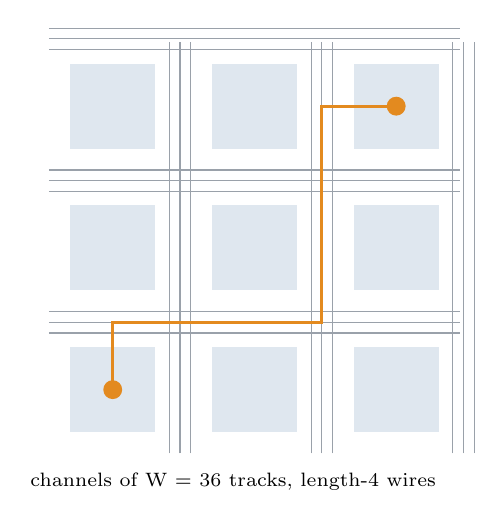
\begin{tikzpicture}[x=9mm,y=9mm]
      \foreach \x in {0,1,2} \foreach \y in {0,1,2}
        { \fill[bobclb] (\x*2,\y*2) rectangle (\x*2+1.2,\y*2+1.2); }
      \foreach \y in {0,1,2} { \foreach \t in {0,0.15,0.3} \draw[bobmute!60] (-0.3,\y*2+1.4+\t) -- (5.5,\y*2+1.4+\t); }
      \foreach \x in {0,1,2} { \foreach \t in {0,0.15,0.3} \draw[bobmute!60] (\x*2+1.4+\t,-0.3) -- (\x*2+1.4+\t,5.5); }
      \draw[bobamber, very thick] (0.6,0.6) -- (0.6,1.55) -- (3.55,1.55) -- (3.55,4.6) -- (4.6,4.6);
      \fill[bobamber] (0.6,0.6) circle (1.2mm); \fill[bobamber] (4.6,4.6) circle (1.2mm);
      \node[font=\scriptsize, fill=white, inner sep=1pt] at (2.3,-0.7) {channels of W = 36 tracks, length-4 wires};
    \end{tikzpicture}
  \end{columns}
\end{frame}

% =============================================================================
\section{Configuration}
\begin{frame}{How a configuration gets in: JTAG and the TAP}
  \begin{columns}[c]
    \column{0.5\textwidth}
    \small
    \begin{itemize}
      \item Four wires: TCK, TMS, TDI, TDO; one bit per clock, \textbf{TCK = 1 MHz} (constrained and proven on the board, M25)
      \item The TAP is the IEEE 1149.1 16-state machine; a 6-bit \textbf{instruction} picks which register TDI feeds
      \item AMD's codes where AMD has them, so the stream looks like a 7-series configuration
    \end{itemize}
    \column{0.48\textwidth}
    \scriptsize
    \begin{tabular}{@{}lll@{}}
      \toprule
      instruction & code & register \\
      \midrule
      IDCODE & 001001 & 32 bits \\
      CFG\_IN & 000101 & packet stream in \\
      CFG\_OUT & 000100 & words out \\
      JPROGRAM & 001011 & clear everything \\
      JSTART & 001100 & startup sequence \\
      CHAIN\_IN & 110101 & whole memory (bob's own) \\
      CAPTURE & 100010 & every user flip-flop \\
      \bottomrule
    \end{tabular}
  \end{columns}
\end{frame}

% =============================================================================
\begin{frame}{The packet stream (after AMD UG470, chapter 5)}
  \small
  \begin{columns}[T]
    \column{0.47\textwidth}
    \ttfamily\scriptsize
    \begin{tabular}{@{}ll@{}}
      FFFFFFFF & dummy \\
      \textcolor{bobamber}{AA995566} & \textcolor{bobamber}{sync word} \\
      30008001 00000007 & CMD = RCRC \\
      30018001 0B025093 & IDCODE check \\
      30002001 00000000 & FAR = 0 \\
      30008001 00000001 & CMD = WCFG \\
      30004000 50000850 & FDRI, 2\,128 words \\
      \textrm{\dots\ 532 frames \dots} & \\
      30000001 A69CAB08 & CRC-32C check \\
      30008001 00000003/5 & LFRM, START \\
    \end{tabular}
    \column{0.5\textwidth}
    \begin{itemize}
      \item The parser \alert{hunts} for the sync word bit by bit, then reads 32-bit words
      \item \textbf{Type-1} header: opcode, register, count; \textbf{type-2}: a 27-bit count for the frame data
      \item Registers: CRC, FAR, FDRI, FDRO, CMD, STAT, IDCODE (7-series addresses)
      \item \textbf{CRC-32C} over \{register, data\} of every write: one wrong bit and startup is refused
      \item The \texttt{counter} example: 2\,154 words
    \end{itemize}
  \end{columns}
\end{frame}

% =============================================================================
\begin{frame}{Frames: how the memory is cut up, and where each lands}
  \begin{columns}[c]
    \column{0.52\textwidth}
    \centering
    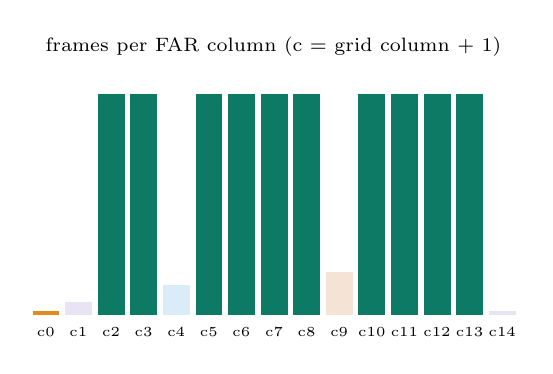
\begin{tikzpicture}[x=3.6mm,y=0.55mm]
      % frames per FAR column: c0..c14
      \foreach \c/\n/\col in {0/1/bobamber,1/3/bobio,2/51/bobteal,3/51/bobteal,4/7/bobbram,5/51/bobteal,6/51/bobteal,7/51/bobteal,8/51/bobteal,9/10/bobdsp,10/51/bobteal,11/51/bobteal,12/51/bobteal,13/51/bobteal,14/1/bobio}
        { \fill[\col] (\c*1.15,0) rectangle (\c*1.15+0.95,\n); \node[font=\tiny] at (\c*1.15+0.47,-4) {c\c}; }
      \node[font=\scriptsize, align=center] at (8.5,62) {frames per FAR column (c = grid column + 1)};
    \end{tikzpicture}
    \column{0.46\textwidth}
    \small
    \begin{itemize}
      \item A \textbf{frame} = 4 words = 128 bits, the unit of writing and reading
      \item \textbf{532 frames}, column-major like 7-series: a CLB column takes 51, BRAM 7, DSP 10, control 1
      \item \textbf{FAR} = block type, column, minor; it counts up by itself, so one FDRI packet fills the chip
      \item A CLB tile = 5 frames: crossbar and flags, two truth-table frames, more crossbar, routing
      \item The \texttt{counter} needs only 26 non-zero frames
    \end{itemize}
  \end{columns}
\end{frame}

% =============================================================================
\begin{frame}{The configuration ``brain'' and where the bits end up}
  \centering
  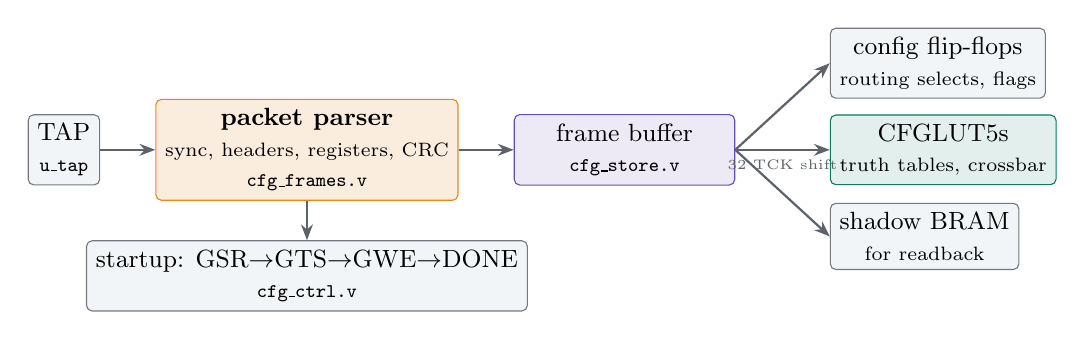
\begin{tikzpicture}[node distance=5mm and 7mm, font=\small]
    \node[blk] (tap) {TAP\\\scriptsize\texttt{u\_tap}};
    \node[hot, right=of tap, minimum width=30mm] (par) {\textbf{packet parser}\\\scriptsize sync, headers, registers, CRC\\\scriptsize\texttt{cfg\_frames.v}};
    \node[blk, below=of par] (ctrl) {startup: GSR$\rightarrow$GTS$\rightarrow$GWE$\rightarrow$DONE\\\scriptsize\texttt{cfg\_ctrl.v}};
    \node[cfg, right=of par, minimum width=28mm] (store) {frame buffer\\\scriptsize\texttt{cfg\_store.v}};
    \node[blk, right=12mm of store, yshift=11mm] (ff) {config flip-flops\\\scriptsize routing selects, flags};
    \node[acc, right=12mm of store] (lut) {CFGLUT5s\\\scriptsize truth tables, crossbar};
    \node[blk, right=12mm of store, yshift=-11mm] (sh) {shadow BRAM\\\scriptsize for readback};
    \draw[arr] (tap) -- (par); \draw[arr] (par) -- (ctrl); \draw[arr] (par) -- (store);
    \draw[arr] (store.east) -- (ff.west); \draw[arr] (store.east) -- node[below,font=\tiny,sloped]{32 TCK shift} (lut.west); \draw[arr] (store.east) -- (sh.west);
  \end{tikzpicture}
  \vspace{2mm}
  \small
  \begin{columns}[T]
    \column{0.48\textwidth}
    \begin{itemize}
      \item \textbf{CFGLUT5 trick} (after ZUMA, Brant \& Lemieux, FCCM 2012, M22): truth tables and crossbar live \emph{in} the host's shift-in LUTs: a CLB went from 469 LUTs + 424 FFs to 193 LUTs + 48 FFs
    \end{itemize}
    \column{0.48\textwidth}
    \begin{itemize}
      \item \textbf{Shadow readback} (M21): readback reads a BRAM copy, removing a 128-bit, 256-way multiplexer, about 11\,800 host LUTs and the worst congestion
    \end{itemize}
  \end{columns}
\end{frame}

% =============================================================================
\begin{frame}{Changing a running design, and time travel}
  \begin{columns}[T]
    \column{0.5\textwidth}
    \textbf{Partial reconfiguration} (M14)
    \small
    \begin{itemize}
      \item AGHIGH freezes the user clock; only the \alert{frames that differ} are written; LFRM releases after the CRC matches
      \item Every register keeps its state while the logic around it changes
      \item \texttt{./bob load new.bit --partial}
    \end{itemize}
    \column{0.5\textwidth}
    \textbf{Time-travel debugging} (M25, after Attia \& Betz, TRETS 2022)
    \small
    \begin{itemize}
      \item \textbf{Save}: CAPTURE every flip-flop of a frozen design
      \item \textbf{Restore}: INIT bits := snapshot, then UG470 \textbf{GRESTORE}, then INIT back, verified while frozen
      \item \textbf{Hand-off}: run a snapshot on in the simulator and put the result back on the chip
      \item \texttt{./bob snap save | restore | sim}
    \end{itemize}
  \end{columns}
  \vspace{3mm}
  \centering
  \src{Board test M25: a counter taken 5 $\rightarrow$ 11 $\rightarrow$ back to 5 $\rightarrow$ 8, and a simulator hand-off +4 $\rightarrow$ 12.}
\end{frame}

% =============================================================================
\section{The tool chain}
\begin{frame}{The tool chain: Verilog to a running design}
  \centering
  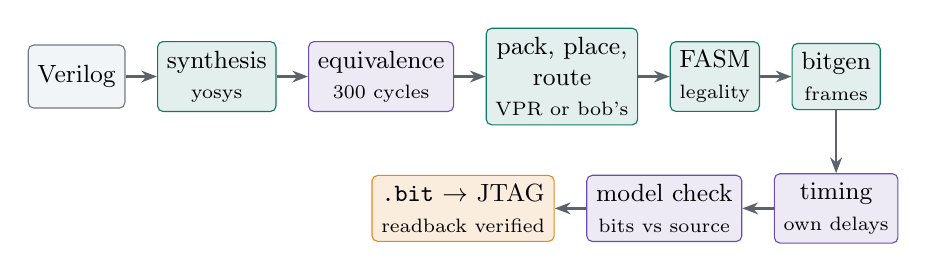
\begin{tikzpicture}[node distance=4mm, font=\small]
    \node[blk] (v) {Verilog};
    \node[acc, right=of v] (sy) {synthesis\\\scriptsize yosys};
    \node[cfg, right=of sy] (eq) {equivalence\\\scriptsize 300 cycles};
    \node[acc, right=of eq] (pr) {pack, place,\\route\\\scriptsize VPR or bob's};
    \node[acc, right=of pr] (fa) {FASM\\\scriptsize legality};
    \node[acc, right=of fa] (bi) {bitgen\\\scriptsize frames};
    \node[cfg, below=8mm of bi] (tm) {timing\\\scriptsize own delays};
    \node[cfg, left=of tm] (mo) {model check\\\scriptsize bits vs source};
    \node[hot, left=of mo] (ld) {\texttt{.bit} $\rightarrow$ JTAG\\\scriptsize readback verified};
    \draw[arr] (v)--(sy); \draw[arr] (sy)--(eq); \draw[arr] (eq)--(pr); \draw[arr] (pr)--(fa); \draw[arr] (fa)--(bi);
    \draw[arr] (bi)--(tm); \draw[arr] (tm)--(mo); \draw[arr] (mo)--(ld);
  \end{tikzpicture}
  \vspace{3mm}
  \small
  \begin{itemize}
    \item One command: \texttt{./bob build design.v}, then \texttt{./bob load design.bit} (or \texttt{./bob run design.v})
    \item \alert{Every stage is checked before the next}: the netlist against the source, the FASM against the device, the bits against a cycle model, the load against a readback
    \item Example \texttt{wide.v}: 16 generic cells $\rightarrow$ 39 bob cells (7 LUTs, 12 adder bits, 20 FFs) $\rightarrow$ 5 CLBs $\rightarrow$ 22 routed nets $\rightarrow$ 247 FASM lines
  \end{itemize}
\end{frame}

% =============================================================================
\begin{frame}{bob's own place and route (M12a)}
  \begin{columns}[c]
    \column{0.55\textwidth}
    \small
    \begin{itemize}
      \item Written from the papers, on the same netlist and rr graph as VPR
      \item \textbf{Packing} with VPR's pack patterns; \textbf{placement} by simulated annealing on half-perimeter wirelength; \textbf{routing} by PathFinder negotiated congestion
      \item Same outputs as VPR, so FASM, bitgen and the board do not know which one ran
      \item \texttt{--pnr python}: no Docker needed
    \end{itemize}
    \column{0.43\textwidth}
    \centering
    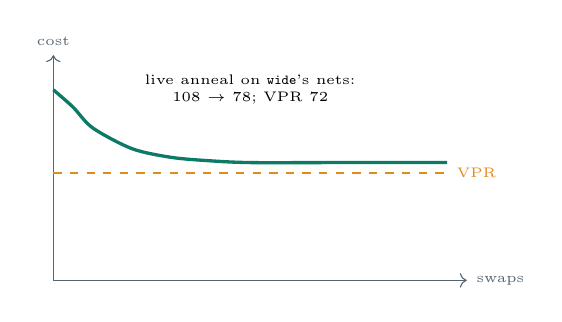
\begin{tikzpicture}[x=5mm,y=2.2mm]
      \draw[->,bobmute] (0,0) -- (10.5,0) node[right,font=\tiny]{swaps};
      \draw[->,bobmute] (0,0) -- (0,13) node[above,font=\tiny]{cost};
      \draw[bobteal, very thick] plot[smooth] coordinates {(0,11) (0.5,10) (1,8.8) (2,7.6) (3,7.1) (4,6.9) (5,6.8) (7,6.8) (10,6.8)};
      \draw[bobamber, dashed] (0,6.2) -- (10,6.2) node[right,font=\tiny]{VPR};
      \node[font=\tiny, align=center] at (5,11) {live anneal on \texttt{wide}'s nets:\\108 $\rightarrow$ 78; VPR 72};
    \end{tikzpicture}
    \vspace{1mm}

    \kpi{0.93$\times$}{VPR's wirelength, same netlists}
  \end{columns}
\end{frame}

% =============================================================================
\section{Timing}
\begin{frame}{Timing without a timing model}
  \begin{columns}[T]
    \column{0.5\textwidth}
    \textbf{The problem}
    \small
    \begin{itemize}
      \item An \emph{unconfigured} fabric is a mesh of combinational loops: Vivado cannot time it (M16, M21 builds missed timing on paths that can never exist)
      \item So the XDC relaxes the fabric's paths, and bob times each design itself
    \end{itemize}
    \textbf{The contract} (M21)
    \begin{itemize}
      \item \texttt{timing.py} walks the \emph{configured} routing and sums per-hop delays
      \item Every build \emph{and every load} is refused unless the critical path fits the clock spacing
    \end{itemize}
    \column{0.48\textwidth}
    \textbf{Measured delays} (after M25)
    \small
    \begin{itemize}
      \item Timed on the routed M25 design, standalone (\texttt{delays.tcl}, no rebuild): 176 clean hops
    \end{itemize}
    \centering
    \begin{tabular}{@{}lcc@{}}
      \toprule
      hop & estimate & measured \\
      \midrule
      routing mux & 3.61 ns & 4.60 ns \\
      input mux & 2.06 ns & 4.65 ns \\
      crossbar & 3.61 ns & 3.01 ns \\
      \bottomrule
    \end{tabular}
    \vspace{1mm}

    \src{A per-design user clock (M20); on silicon the computed clock had 4.5--5$\times$ margin.}
  \end{columns}
\end{frame}

% =============================================================================
\section{Software}
\begin{frame}{Software: the command line and bob studio}
  \begin{columns}[T]
    \column{0.48\textwidth}
    \textbf{\texttt{./bob}}
    \small
    \begin{itemize}
      \item \texttt{build}, \texttt{load}, \texttt{run}, \texttt{new}, \texttt{snap}, \texttt{info}, \texttt{fasm}
      \item \texttt{doctor}: checks yosys, iverilog, Docker, the Pico and the board's IDCODE
      \item Failures name the stage, the file and line, show the line, and say what to do
      \item \texttt{--probe fake}: the whole flow with the board simulated in software
    \end{itemize}
    \column{0.5\textwidth}
    \textbf{bob studio} (M17--M19, desktop app)
    \small
    \begin{itemize}
      \item Laid out like Vivado: sources, editor, flow navigator, messages
      \item Start page, one-click \textbf{Build \& Program}
      \item Device view of the placement and routes; pin planner; block designs with 14 IP cores
      \item Waveform viewer over boundary scan (a logic analyser needing no extra logic)
    \end{itemize}
  \end{columns}
  \vspace{2mm}
  \centering
  \src{Same engine (\texttt{flow.py}) behind the CLI and the studio; tests require both to write byte-identical bitstreams.}
\end{frame}

% =============================================================================
\section{Verification}
\begin{frame}{Verification: every layer checked by something independent}
  \centering
  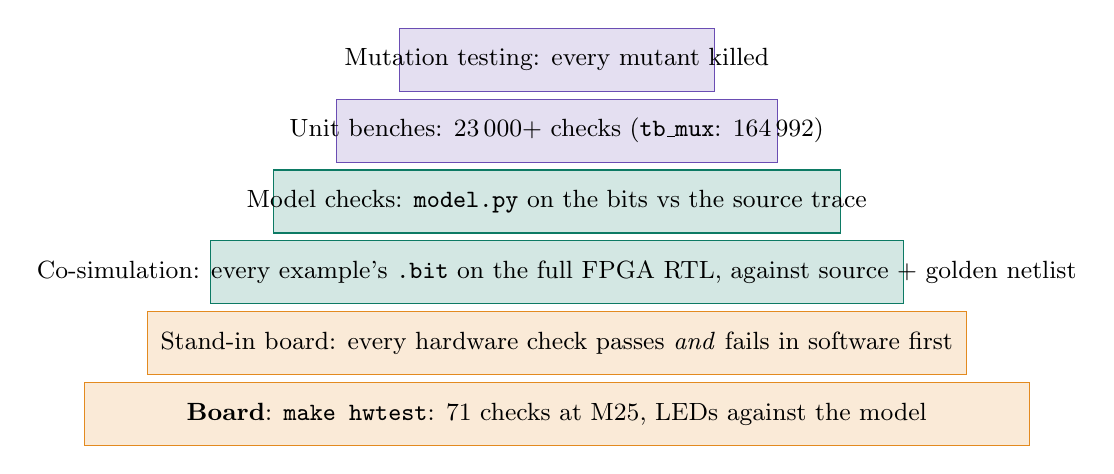
\begin{tikzpicture}[font=\small, x=1mm, y=1mm]
    \foreach \w/\y/\t/\c in {
      120/0/{\textbf{Board}: \texttt{make hwtest}: 71 checks at M25, LEDs against the model}/bobamber,
      104/9/{Stand-in board: every hardware check passes \emph{and} fails in software first}/bobamber,
       88/18/{Co-simulation: every example's \texttt{.bit} on the full FPGA RTL, against source + golden netlist}/bobteal,
       72/27/{Model checks: \texttt{model.py} on the bits vs the source trace}/bobteal,
       56/36/{Unit benches: 23\,000+ checks (\texttt{tb\_mux}: 164\,992)}/bobviolet,
       40/45/{Mutation testing: every mutant killed}/bobviolet}
      { \fill[\c!18] (-\w/2,\y) rectangle (\w/2,\y+8); \draw[\c] (-\w/2,\y) rectangle (\w/2,\y+8); \node at (0,\y+4) {\t}; }
  \end{tikzpicture}
  \vspace{2mm}

  \small Plus 585 pytest tests (flow, tools, Vivado scripts on a Tcl stub, CLI wording) and lint. A test that cannot fail proves nothing: the M8 counter trace was all zeros until a check caught it.
\end{frame}

% =============================================================================
\section{Growing the grid}
\begin{frame}{Growing the grid: 16 to 400 LUTs on the same chip}
  \begin{columns}[c]
    \column{0.55\textwidth}
    \centering
    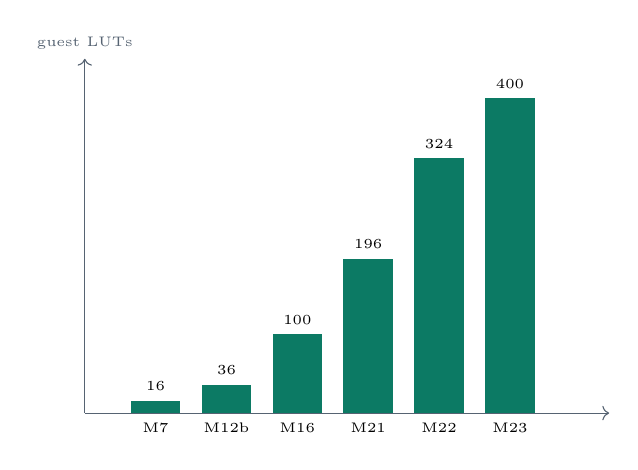
\begin{tikzpicture}[x=9mm,y=0.1mm]
      \draw[->,bobmute] (0,0) -- (7.4,0);
      \draw[->,bobmute] (0,0) -- (0,450) node[above,font=\tiny]{guest LUTs};
      \foreach \i/\m/\v in {1/M7/16,2/M12b/36,3/M16/100,4/M21/196,5/M22/324,6/M23/400}
        { \fill[bobteal] (\i-0.35,0) rectangle (\i+0.35,\v); \node[font=\tiny,above] at (\i,\v) {\v}; \node[font=\tiny,below] at (\i,0) {\m}; }
    \end{tikzpicture}
    \column{0.43\textwidth}
    \small
    Each step paid for by removing overhead, not adding chip:
    \begin{itemize}
      \item M12b: the chain streamed through one frame buffer ($-$3.6k LUT, $-$4.8k FF)
      \item M21: 4-element clusters; readback from a BRAM shadow
      \item M22: LUT contents in CFGLUT5
      \item M23: a sweep found the real wall (\alert{SLICEM} slices); OR roots and LUT6/MUXF7/MUXF8 routing muxes reached \textbf{10 $\times$ 10}
    \end{itemize}
  \end{columns}
\end{frame}

% =============================================================================
\section{Results}
\begin{frame}{Hardware results, milestone by milestone}
  \centering
  \scriptsize
  \begin{tabular}{@{}llrrrr@{}}
    \toprule
    M & what & board checks & host LUTs & slices & WNS \\
    \midrule
    M7  & fabric generated from VPR's rr graph, 16 CLBs & 26/26 & 7\,670 & & $-$1102 ns$^*$ \\
    M13 & UG470 frames and packets & 39/39 & 11\,607 & & +0.877 ns \\
    M15 & BRAM contents as frames; 36 CLBs & 48/48 & 10\,411 & & +0.585 ns \\
    M16 & 100 single-LUT CLBs & 50/50 & 20\,498 & & +0.667 ns \\
    M21 & cluster CLB, BRAM shadow, timing contract & 66/66 & 35\,882 & & +0.570 ns \\
    M22 & CFGLUT5 LUTs, 81 CLBs & 65/67$^\dagger$ & 38\,184 & & +0.172 ns \\
    M23 & 10 $\times$ 10 = 100 CLBs, 400 LUTs & 68/68 & 36\,710 & 88.0\% & +0.048 ns \\
    M24 & Double Duty elements & 69/69 & 38\,193 & 85.5\% & +0.562 ns \\
    M25 & time travel, TCK 1 MHz & \textbf{71/71} & 38\,198 & 86.8\% & +0.732 ns \\
    \bottomrule
  \end{tabular}
  \vspace{2mm}

  \src{$^*$ hardware correct; the timing was analysed and fixed at M13. $^\dagger$ the two failing live checks passed 12/12 on rerun.}
\end{frame}

% =============================================================================
\begin{frame}{Problems met, and what they taught}
  \small
  \begin{columns}[T]
    \column{0.5\textwidth}
    \begin{itemize}
      \item \textbf{Vivado crashed} in synthesis with the XDC or \texttt{keep\_hierarchy}: synthesis now runs without both
      \item \textbf{An empty fabric cannot be timed}: loops everywhere. Answer: relax it in Vivado, time each design from its own bits
      \item \textbf{12 $\times$ 11 did not place}: a dual-output CFGLUT5 takes \emph{two} LUT sites
      \item \textbf{A load order made a ring oscillator}: frames now load flags before truth tables before the crossbar
    \end{itemize}
    \column{0.5\textwidth}
    \begin{itemize}
      \item \textbf{Delay extraction} crashed Vivado, then found nothing: nets renamed inside muxes; now a standalone, bounded, name-proof script
      \item \textbf{A RISC-V CPU (SERV) inside bob}: the logic fits (186 LUTs) but it does not route (4 overused pins): \alert{routing, not logic, is the limit}
      \item Faster TCK: 100 kHz $\rightarrow$ 1 MHz only after constraining and proving it (board regression 10 $\rightarrow$ 8 min)
    \end{itemize}
  \end{columns}
\end{frame}

% =============================================================================
\begin{frame}{How bob compares}
  \centering
  \small
  \begin{tabular}{@{}lllll@{}}
    \toprule
     & \textbf{bob} & OpenFPGA & ZUMA & Aegis \\
    \midrule
    what it is & FPGA + controller + tools & fabric generator + flow & overlay & fabric generator \\
    runs on & PYNQ-Z2, board-tested & silicon (tape-out) & a commercial FPGA & silicon (PDK) \\
    routing from VPR's rr graph & yes & yes & VPR-based & own generator \\
    configuration & UG470 frames + chain & chain, frames, banks & host LUTRAM & one scan chain \\
    partial reconf., state kept & yes, proven & protocol only & -- & -- \\
    LUT tables in host LUTRAM & yes (CFGLUT5) & n/a & yes & n/a \\
    scale & 400 LUTs & many architectures & large overlays & whole devices \\
    \bottomrule
  \end{tabular}
  \vspace{2mm}

  \src{Detailed comparison: \texttt{docs/project/GUIDE.md}, section 5.}
\end{frame}

% =============================================================================
\begin{frame}{Documentation and teaching material}
  \begin{columns}[T]
    \column{0.5\textwidth}
    \small
    \textbf{Four animated volumes} (\texttt{docs/learn/}), each built from the chip's own data:
    \begin{enumerate}
      \item \emph{Bit by bit}: gates, LUTs, flip-flops, routing
      \item \emph{Layer by layer}: bob built up one layer at a time
      \item \emph{Frame by frame}: one configuration from the cable through the TAP and the packet parser to its tiles
      \item \emph{Tool by tool}: one design through every tool, with a live annealing placer
    \end{enumerate}
    \column{0.48\textwidth}
    \small
    \textbf{Reference documents}
    \begin{itemize}
      \item \texttt{GETTING\_STARTED.md}: a first design in ten minutes
      \item \texttt{bitstream-format.md}: the format, bit by bit
      \item \texttt{GUIDE.md}: every part, what/why/how to change it
      \item \texttt{REPORT.md}: the whole project, measured
      \item \texttt{docs/hwtest/}: a checklist per milestone
    \end{itemize}
  \end{columns}
\end{frame}

% =============================================================================
\section{Limits and future work}
\begin{frame}{Limits and future work}
  \begin{columns}[T]
    \column{0.48\textwidth}
    \textbf{Known limits}
    \small
    \begin{itemize}
      \item Thin routing (fc\_in 0.10): bigger designs such as a soft CPU do not route
      \item LUT, carry and flip-flop delays still estimated
      \item One clock domain for guest designs; CAPTURE covers CLB registers only
      \item Readback reads the shadow, not the cells
      \item 10 $\times$ 10 is this CLB's ceiling on the XC7Z020
    \end{itemize}
    \column{0.5\textwidth}
    \textbf{Next}
    \small
    \begin{itemize}
      \item \textbf{Configuration from the ARM core} over AXI: loads in milliseconds, bob as a PYNQ overlay
      \item \textbf{Scrubbing}: readback CRC and frame ECC, repairing a flipped bit while the design runs
      \item \textbf{A built-in logic analyser} into a BRAM
      \item \textbf{Richer routing}, sized by a sweep, for bigger designs
      \item Timing-driven placement on the measured delays
    \end{itemize}
  \end{columns}
\end{frame}

% =============================================================================
\begin{frame}{Summary}
  \begin{itemize}
    \item A complete FPGA, \textbf{bob}, runs inside a Zynq XC7Z020: 400 LUT6, 2 BRAM, 2 DSP, 44 pads, generated from VPR's own routing graph
    \item Configured the way AMD configures its chips: \textbf{UG470 packets and frames} over JTAG, with CRC, readback, partial reconfiguration and time travel
    \item Its own \textbf{tool chain} from Verilog to the board, every step checked, with its own timing sign-off
    \item Grown from \textbf{16 to 400 LUTs} on the same chip by removing overhead: frame streaming, clusters, a shadow for readback, LUTs in host LUTRAM
    \item Proven on the board at every one of \textbf{26 milestones}; M25: 71/71
  \end{itemize}
  \vspace{4mm}
  \centering
  \kpi{400}{LUT6 in 100 CLBs}\qquad
  \kpi{68\,096}{configuration bits}\qquad
  \kpi{71/71}{board checks}\qquad
  \kpi{0.93$\times$}{VPR wirelength (own PnR)}
\end{frame}

% =============================================================================
\begin{frame}[plain]
  \centering
  \vspace{18mm}
  {\Huge\bfseries Thank you}\\[6mm]
  {\large Questions?}\\[12mm]
  \src{Live demo: \texttt{./bob run work/examples/counter/counter.v} \quad$\cdot$\quad bob studio \quad$\cdot$\quad \texttt{docs/learn/}}
\end{frame}

\end{document}
